\documentclass{beamer}
\usepackage{listings}

%Information to be included in the title page:
\title{Performance Analysis on Covid-19 Models with Discontinuities and Efficient Defect Control for Initial Value ODE solvers}
\author{Humaid M. Agowun}
\institute{Saint Mary's University}
\date{2022}

\begin{document}

\frame{\titlepage}


\section{Covid19 modelling}
\begin{frame}
\frametitle{Modelling Covid-19 using an SEIR Ordinary Differential Equation (ODE) system}

\begin{equation}
\frac{\textit{d}S}{\textit{dt}} = \mu N - \mu S - \frac{\beta}{N}IS, \nonumber
\end{equation}

\begin{equation}
\frac{\textit{d}E}{\textit{dt}} = \frac{\beta}{N}IS - \alpha E - \mu E, \nonumber
\end{equation}

\begin{equation}
\frac{\textit{d}I}{\textit{dt}} = \alpha E - \gamma I - \mu I, \nonumber
\end{equation}

\begin{equation}
\frac{\textit{d}R}{\textit{dt}} = \gamma I - \mu R \nonumber
\end{equation} 

S(t) is the number of susceptible individuals, 
E(t) is the number of exposed individuals, 
I(t) is the number of infected individuals and 
R(t) is the number of recovered individuals at a point in time. 
\end{frame}

\begin{frame}[fragile]
\frametitle{Solving the model}
We define the ODE problem as a model function, give some initial values, and the times at which to sample the solutions y(t) = (S(t), E(t), I(t), R(t))

\begin{lstlisting}
function f(t, y):
    (S, E, I, R) = y
    // define parameters ...
    dSdt = mu*N - mu*S - (beta/N)*I*S
    dEdt = (beta/N)*I*S - alpha*E - mu*E
    dIdt = alpha*E - gamma*I - mu*I
    dRdt = gamma*I - mu*R
    return (dSdt, dEdt, dIdt, dRdt)

E0 = 103; I0 = 1; R0 = 0; N = 37.741 * (10**6)
S0 = N - (E0 + I0 + R0)
y0 = (S0, E0, I0, R0)
t_eval = [0, 1, 2, ..., 95]
tol = 1e-6

res = ode_solver(f, t_eval, y0, tol)
plot(t_eval, res)
\end{lstlisting}
\end{frame}

\begin{frame}
\frametitle{Typical plot to solutions to an SEIR model}
\begin{figure}[H]
\centering
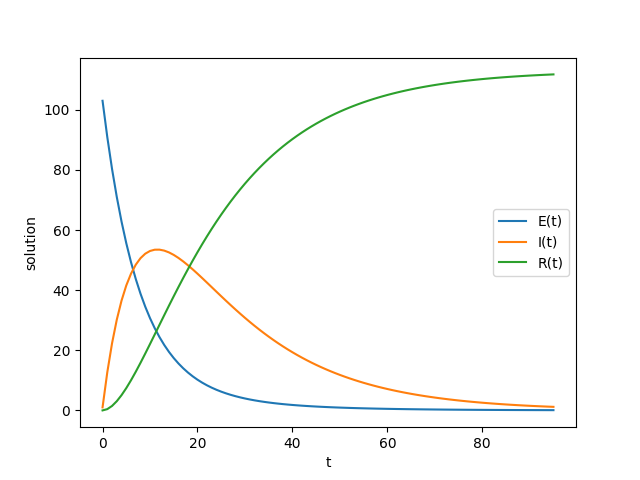
\includegraphics[width=0.7\linewidth]{./figures/SEIR}
\caption{Solutions to the SEIR model. Note that S(t) is taken to be large enough that it appears infinite and cannot be plotted alongside E(t), I(t) and R(t)}
\label{fig:SEIR}
\end{figure}
\end{frame}

\subsection{time-dependent discontinuity}
\begin{frame}[fragile]
\frametitle{Real-life models and Preventive Measures}
Real-life model = vary the $\beta$ parameter to model the introduction of Covid-19 measures.
The if-statement introduces a discontinuity.
\begin{lstlisting}
function f(t, y):
    (S, E, I, R) = y
    // parameters ...
    if (t < 27): 
        beta = 0.9 # no measures
    else: 
        beta = 0.005 # severe drop in transmission dues to measures
    // ...
    return (dSdt, dEdt, dIdt, dRdt)
\end{lstlisting}
\end{frame}

\begin{frame}
\frametitle{How modern ODE solvers work}
ODE solvers work by taking a sequence of time steps.

Using an initial step-size $h$, solver takes a step from $t_0$ to $t_0 + h$ using some evaluations of the function $f(t, y)$. 
\newline \newline
% Modern solvers use error control in that after taking this step to $t_0 + h$, they calculate an error estimate. 
Calculate error estimate at the end of the step.
If that error estimate is within the user provided tolerance, accept the step.
Else, retake the step with a smaller step-size (e.g, $\frac{h}{2}$).
\newline \newline
% the error is proportional to the size of the step so a smaller step-size will produce a smaller error.
Modern solvers also increase the step-size for the next step if the error-estimate is much smaller than the tolerance.
\newline \newline
A solver that employs this type of algorithm is called an error control solver.
\end{frame}

\begin{frame}
\frametitle{Thrashing}
The if-statement makes $f(t, y(t))$ discontinuous.
This causes difficulties for ODE solvers.
\emph{Error control} solvers observed to solve discontinuous problem.
\begin{figure}[H]
\centering
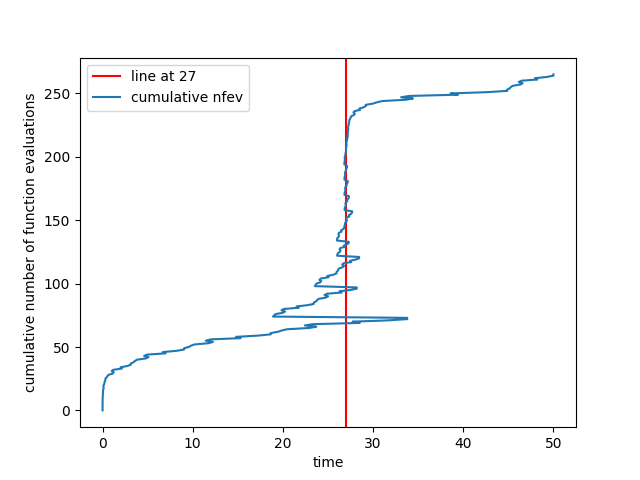
\includegraphics[width=0.7\linewidth]{./figures/ode_thrashing}
\caption{Number of function evaluations spike at a discontinuity in a process called `THRASHING', i.e., repeated step-size reductions.}
\label{fig:ode_thrashing}
\end{figure}
\end{frame}

\begin{frame}
\frametitle{Impacts of time-dependent discontinuity}
Thrashing impacts the efficiency because the solvers are forced to take very small steps.
Thrashing impacts the accuracy, as some solvers accept a wrong step.
\begin{figure}[H]
\centering
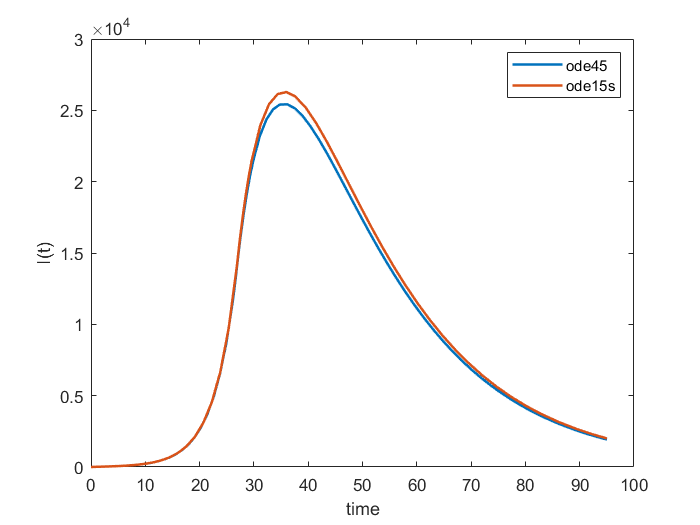
\includegraphics[width=0.7\linewidth]{./figures/time_discontinuity_matlab}
\caption{Robust MATLAB solvers giving varying solutions to discontinuous problems.}
\label{fig:time_discontinuity_matlab}
\end{figure}
\end{frame}

\begin{frame}[fragile]
\frametitle{Solution to time-dependent discontinuity}
Use a COLD START at the discontinuity. \newline 
No values from the previous call impact the new call. \newline
Each call solves a continous subproblem.
\begin{lstlisting}[language=Python]
y0_1 = (S0, E0, I0, R0)
tspan1 = [0, ..., 27]
sol1 = ode(y0_1, f_0_9, tspan1, 1e-6)

y0_2 = last_row(sol1)
tspan2 = [27, ..., 95]
sol2 = ode(y0_2, f_0_005, tspan2, 1e-6)

sol = concat(sol1, sol2)
\end{lstlisting}
\end{frame}

\begin{frame}
\frametitle{Impacts of cold starts}
Cold starts solve the efficiency and accuracy problems.
\begin{table}[H]
\caption {Python Efficiency data for the time-dependent discontinuity problem - number of function evaluations} 
\label{tab:time_discontinuity_Py} 
\begin{center}
\begin{tabular}{ c c c }
method & no discontinuity handling & with discontinuity handling \\ 
lsoda & 162 & 124 \\
rk45 & 134 & 130 \\
bdf & 202 & 146 \\
radau & 336 & 220 \\
dop853 & 329 & 181 \\
rk23 & 152 & 127 \\
\end{tabular}
\end{center}
\end{table}
The solution is more accurate as well. For example MATLAB ode45 accurately solves the problem when cold starts are used.
\end{frame}

\begin{frame}
\frametitle{Matlab solvers accurately solve the time-dependent discontinuity model when using a cold start.}
\begin{figure}[H]
\centering
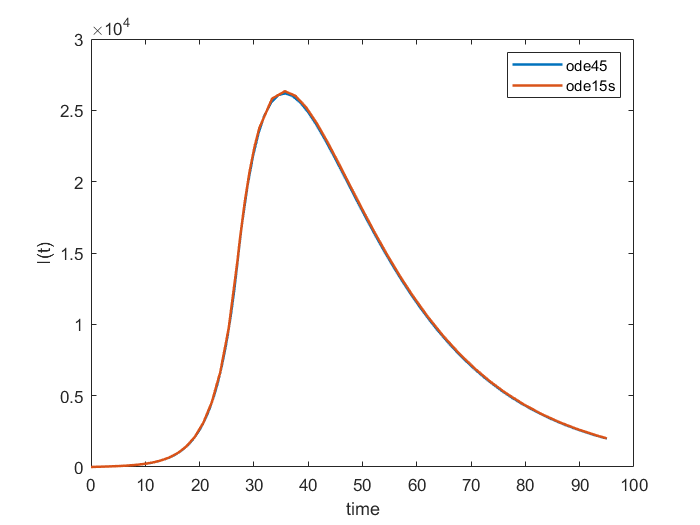
\includegraphics[width=0.7\linewidth]{./figures/solve_time_discontinuity_matlab}
\caption{Robust MATLAB solvers giving accurate solutions to discontinuous problems.}
\label{fig:solve_time_discontinuity_matlab}
\end{figure}
\end{frame}

\subsection{State-dependent discontinuity}
\begin{frame}[fragile]
\frametitle{State-dependent discontinuity}
Previously, the if-statement was based on the time.
We are now going to discuss state-dependent discontinuities.
\begin{lstlisting}[language=Python]
measures_implemented = False
direction = "up"
function model_with_if(_, y):
    // ...
    if (direction == "up" and E > 25000):
        measures_implemented = True
        direction = "down"
    elif (direction == "down" and E < 10000):
        measures_implemented = False
        direction = "up"

    if measures_implemented: beta = 0.005 
    else: beta = 0.9
    // ...
    return (dSdt, dEdt, dIdt, dRdt)
\end{lstlisting}
\end{frame}

\begin{frame}
\frametitle{Impacts of the state-dependent discontinuities}
Everytime the value of the parameter $\beta$ changes, there is a discontinuity.
Solvers, even when using sharp tolerances, cannot solve it.
\begin{figure}[H]
\centering
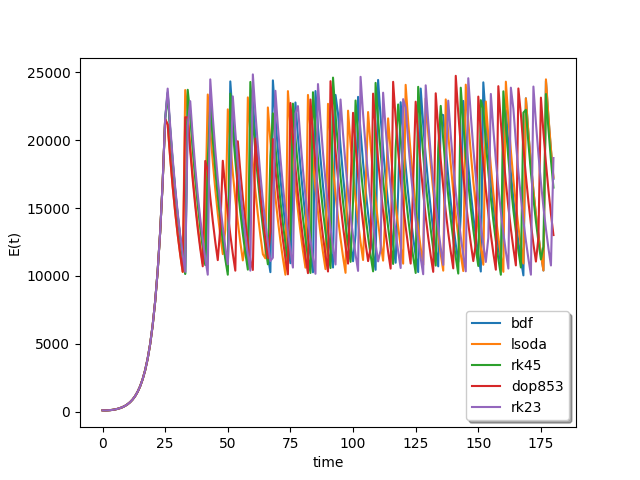
\includegraphics[width=0.7\linewidth]{./figures/state_discontinuity_sharp_py}
\caption{Solutions to the state-dependent problem using the simple approach in Python at a very sharp tolerance.}
\label{fig:state_discontinuity_sharp_py}
\end{figure}
\end{frame}

\begin{frame}
\frametitle{Event detection}
Event detection requires the user to also provide a root function, $g(t, y(t))$, that defines the events.
\newline \newline
The solver will now call the root function at the end of each successful step.
It caches the previous value of the root function and if there is a change in sign between the previous and the current value, it knows that there is a root somewhere within the step.
\newline \newline
The solver will then run a root-finding algorithm (Bisection, BRENT, ...) to detect the location of the root.
\newline \newline
For example, if we want to detect when y is 100, it is sufficient to define the root function as \emph{return (y - 100);}. 
\end{frame}

\begin{frame}[fragile]
\frametitle{Solving the state-dependent discontinuity problem}
\begin{lstlisting}[language=Python]
res = array(); t0 = 0; y0 = (S0, E0, I0, R0)
while t0 < 180:
    tspan = [t0, ..., 180]
    if (measures_implemented):
        sol = ode(f_measures, tspan, 
            y0, events=root_10000)
        measures_implemented = False
    else:
        sol = ode(f_no_measures, tspan, 
            y0, events=root_25000)
        measures_implemented = True
    t0 = extract_last_t(sol)
    y0 = extract_last_row(sol)
    res = concatenate(res, sol)
\end{lstlisting}
In this way, each call to the solver involves a continuous subproblem.
\end{frame}

\begin{frame}
\frametitle{Accuracy of event-detection solution}
Recall that none of the solutions from the solvers in Python were aligned even at a very sharp tolerance.
With event detection, all the solutions are aligned. Thus the accuracy is improved.
\begin{figure}[H]
    \centering
    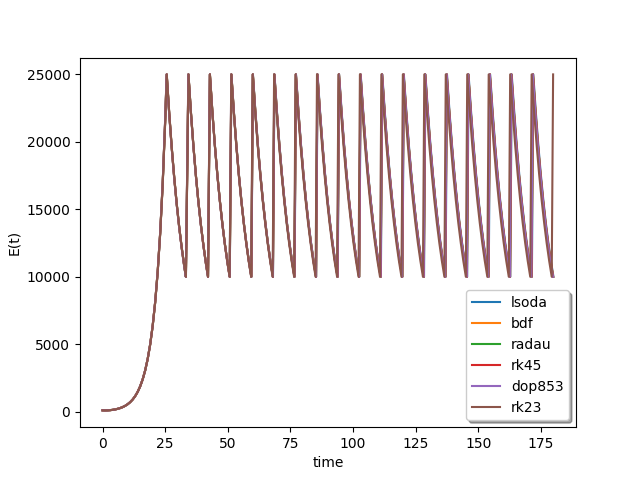
\includegraphics[width=0.7\linewidth]{./figures/solve_state_discontinuity_py}
    \caption{Solutions to the state-dependent problem using event detection in Python.}
    \label{fig:solve_state_discontinuity_py}
    \end{figure}
\end{frame}

\begin{frame}
\frametitle{Efficiency of event detection solution}
\begin{table}[h]
    \caption {Efficiency data for Python state-dependent discontinuity model - number of function evaluations} \label{tab:state_discontinuity_Py}
    \begin{center}
    \begin{tabular}{ c c c c } 
    method & no event & no event with sharp tol. & with event detection \\ 
    lsoda & 2357 & 4282 & 535 \\
    bdf & 2301 & 11794 & 808 \\
    radau & 211 & 74723 & 990 \\
    rk45 & 1484 & 17648 & 674 \\
    dop853 & 11129 & 21131 & 1514 \\
    rk23 & 4307 & 246644 & 589 \\
    \end{tabular}
    \end{center}
\end{table}
Significant reductions in number of function evaluations, even when compared to the default tolerance number of function evaluation. The computed solutions are much more accurate as well.
\end{frame}

\begin{frame}
\frametitle{Summary - Solving discontinuous Covid-19 models}
Time-dependent discontinuity:
Instead of using an if-statement based on the time at which the discontinuity arises, $t_{if}$, integrate in two parts with a cold start between, i.e, integrate $[t_0, t_{if}]$, cold start, then integrate $[t_{if}, t_f]$.
\newline \newline
State-dependent discontinuity:
Instead of using an if-statement based on state thresholds, use root functions that detect when a threshold is reached, integrate until a root is detection, cold start, then integrate after the root with the new model.
\newline \newline
\end{frame}

\section{Efficient Defect control using multistep interpolants}
\begin{frame}
\frametitle{Efficient Defect Control - Introduction}
Error control is only applied at the end of each time step.
Traditional ODE solvers produce continuous solutions by performing interpolation of the discrete solution values.
\begin{figure}[H]
    \centering
    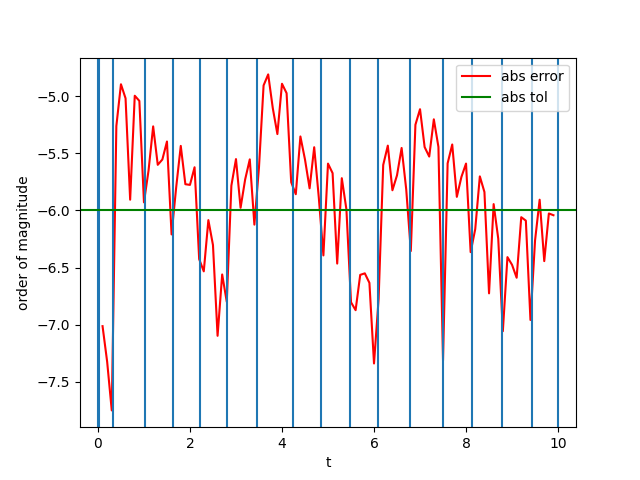
\includegraphics[width=0.7\linewidth]{./figures/no_middle_step_error_control_p3_rk45}
    \caption{Robust Python solver `RK45' produces solutions with errors of one order of magnitude larger than the tolerance within the step.}
    \label{fig:no_middle_step_error_control_p3_rk45}
\end{figure}
\end{frame}

\begin{frame}
\frametitle{Definition of Defect control}
Users of ODE solvers expect that the solution is accurate to the tolerance throughout each step.
The challenge is thus to produce ODE solvers that guarantee accurate continuous solutions. We do so by performing defect control.

The defect, denoted by $\delta(t)$,  is the amount by which the continuous numerical solution, $u(t)$, fails to satify the ODE. 
When the ODE is $y'(t) = f(t, y(t))$, the defect is 
\begin{equation}
\delta(t) = |u'(t) - f(t, u(t))|.
\end{equation}
A defect control solver takes a step using a traditional numerical method, extends the discrete solution to obtain a continuous solution and then samples the maximum defect within the step. If that maximum defect is within the tolerance, it accepts the step, else it rejects it and takes a smaller step.
\newline
In this presentation, we will augment the Classical Runge-Kutta method of $4^{th}$ order with interpolants of order 4, 6 and 8 to provide defect controlled solutions.
\end{frame}

\begin{frame}
\frametitle{More on related work}
Related work to produce a continuous solution is to use a a continuous Runge Kutta method. 
These method perform more stages than traditional discrete Runge-Kutta methods.
In this thesis, we use multistep methods to use no additional function evaluation to produce a continuous solution. This drastically improves the efficiency.
\begin{table}[h]
   \caption {Number of stages for discrete vs continuous RK method} 
   \label{tab:crk_nstages}
   \begin{center}
   \begin{tabular}{ c c c } 
   order   & discrete & continuous \\ 
   4 & 4  & 4  \\ 
   5 & 5  & 6  \\ 
   6 & 6  & 7  \\ 
   7 & 7  & 9  \\ 
   8 & 8  & 13 \\ 
   \end{tabular}
   \end{center}
   \end{table}
\end{frame}

\begin{frame}
\frametitle{HB4}
The Hermite cubic is a popular $4^{th}$ order interpolant.
That is if the space between interpolated data values, $h$, are reduced to $h/10$, we expect the interpolation error over the new set of data values to be $e/10^{4}$, where $e$ was the interpolation error with a spacing of $h$. 

The HB4 scheme constructs and interpolant using both the solution value and derivative at 2 points $x_i$ and $x_{i + 1}$.

\begin{equation}
\label{eqn:HB4}
u(t_i + \theta h) = h_{00}(\theta)y_i +  h_ih_{10}(\theta)f_i + h_{01}(\theta)y_{i + 1} + h_ih_{11}(\theta)f_{i + 1}, 
\end{equation}
\begin{equation}
\label{eqn:HB4_theta}
\theta = (t - t_i) / h_i.
\end{equation}

When $\theta$ is 0, $t_i + \theta h$ is $t_i$.
When $\theta$ is 1, $t_i + \theta h$ is $t_{i + 1}$.
Using the above, we can produce 4 linear systems of 4 equations to derive the 4 cubic polynomials.
\end{frame}

\begin{frame}
\frametitle{RK4 with HB4 controls the defect}
\begin{figure}[H]
    \centering
    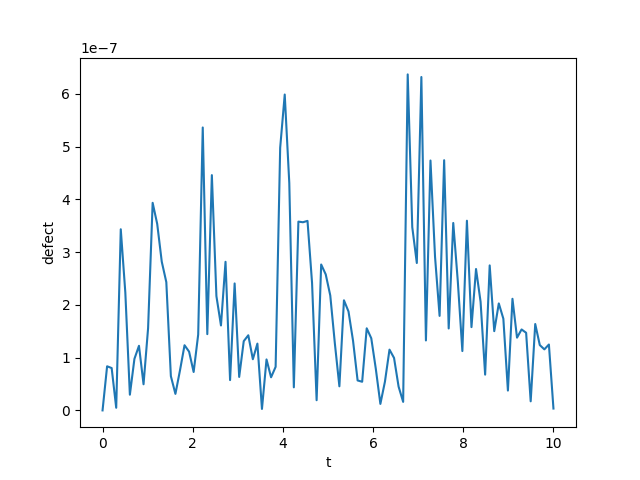
\includegraphics[width=0.7\linewidth]{./figures/rk4_with_hb4_p1_global_defect}
    \caption{Augmenting RK4 with HB4 successfully controls the defect at a tolerance of $10^{-6}$.}
    \label{fig:rk4_with_hb4_p1_global_defect}
\end{figure}
\end{frame}    

\begin{frame}
\frametitle{Issues for RK4 with HB4}
The Hermite cubic, HB4, is an interpolant of $4^{th}$ order.
To perform defect control we need its derivative.
Differentiating a Hermite interpolant decreases the order by 1.
The order of the derivative is 3. 

The interpolation error thus affects the computation of the defect because the numerical solution is $4^{th}$ order but the derivative is of $3^{rd}$ order.
\end{frame}

\begin{frame}
\frametitle{Derivation of HB6 and weight parameters}
HB6 is \emph{multistep}. It will require 3 data points and will be through 2 steps. Those 2 steps may be of different size. 
We thus introduce a weight parameters $\alpha$.
We assume that the step from $x_i$ to $x_{i + 1}$ is of size $h$ but the step from $x_{i - 1}$ to $x_i$ is $\alpha h$. 
The interpolant is based on solution and derivative values from two steps.

\begin{equation}
\begin{split}
u(t_i + \theta h) = d_{0}(\theta) y_{i-1} +  h_id_{1}(\theta)f_{i-1}
+ d_{2}(\theta)y_i  \\   +  h_id_{3}(\theta)f_i
+ d_{4}(\theta)y_{i + 1} + h_id_{5}(\theta)f_{i + 1}, \\
\end{split}
\end{equation}

When $\theta$ is $-\alpha$, $t_i + \theta h$ is $t_{i - 1}$.
When $\theta$ is 0, $t_i + \theta h$ is $t_i$.
When $\theta$ is 1, $t_i + \theta h$ is $t_{i + 1}$.
Using the above, we can produce 6 linear systems of 6 equations to derive the 6 quintic polynomials $d_i(\theta)$.
\end{frame}

\begin{frame}
\frametitle{RK4 with HB6 controls the defect}
\begin{figure}[H]
    \centering
    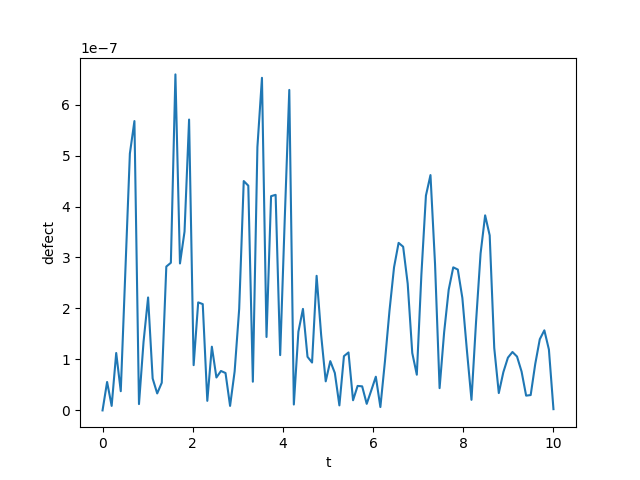
\includegraphics[width=0.7\linewidth]{./figures/rk4_with_hb6_p1_global_defect}
    \caption{Augmenting RK4 with HB6 successfully controls the defect at a tolerance of $10^{-6}$.}
    \label{fig:rk4_with_hb6_p1_global_defect}
\end{figure}
\end{frame}

\begin{frame}
\frametitle{HB6 is more efficient than HB4}
Across the several problems that we used to test RK4 with HB4 and RK4 with HB6, we find that RK4 with HB6 tends to take three times less steps than RK4 with HB4. 

HB6 is of $6^{th}$ and its derivative is of $5^{th}$ order. Thus its interpolation error will be smaller than the numerical solution error.

This is entirely because of having a lower interpolation error.
\end{frame}

\begin{frame}
\frametitle{HB8}
To produce an $8^{th}$ order interpolant, we need to use 4 data points and thus three steps. We thus use two parameters $\alpha$ and $\beta$ such that the step-sizes are $\alpha h$ for the step from $x_{i-2}$ to $x_{i - 1}$, $h$ for the step from $x_{i-1}$ to $x_i$ and $\beta h$ for the step from $x_i$ to $x_{i + 1}$.
The equation for the interpolant is:
\begin{equation}
\begin{split}
u(t_i + \theta h) = d_{0}(\theta)y_{i-2} +  h_id_{1}(\theta)f_{i-2} 
+ d_{2}(\theta)y_{i-1}     +  h_id_{3}(\theta)f_{i-1} \\
+ d_{4}(\theta)y_i     +  h_id_{5}(\theta)f_i 
+ d_{6}(\theta)y_{i + 1} + h_id_{7}(\theta)f_{i + 1}, \\
\end{split}
\end{equation}

When $\theta$ is $-1-\alpha$, $t_i + \theta h$ is $t_{i-2}$.
When $\theta$ is -1, $t_i + \theta h$ is $t_{i-1}$.
When $\theta$ is 0, $t_i + \theta h$ is $t_{i}$
When $\theta$ is $\beta$, $t_i + \theta h$ is $t_{i + 1}$. 
Using the above, we can produce 8 linear systems of 8 equations to derive the 8 septic polynomials $d_i(\theta)$.
\end{frame}

\begin{frame}
\frametitle{RK4 with HB8 controls the defect}
\begin{figure}[H]
    \centering
    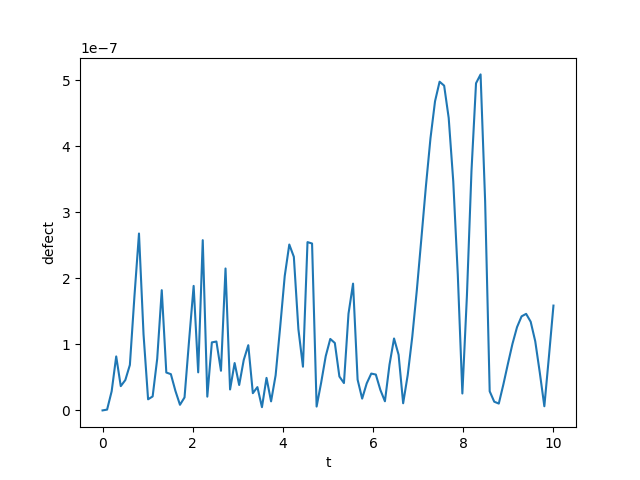
\includegraphics[width=0.7\linewidth]{./figures/rk4_with_hb8_p1_global_defect}
    \caption{Augmenting RK4 with HB8 successfully controls the defect at a tolerance of $10^{-6}$.}
    \label{fig:rk4_with_hb8_p1_global_defect}
\end{figure}
\end{frame}

\begin{frame}
\frametitle{Use of HB8 for higher order Runge-Kutta methods}
RK4 with HB8 is not significantly more efficient than RK4 with HB6. They take about the same number of steps. 
\newline \newline
The main purpose of HB8 is that it can be used to efficiently augment a $6^{th}$ order Runge-Kutta method.
\newline \newline
It can also be used to provide defect control for an $8^{th}$ order Runge-Kutta method though that would not be optimal as the derivative of the interpolant is only of $7^{th}$ order when the discrete solutions are of $8^{th}$ order. 
\end{frame}

\begin{frame}
\frametitle{Summary}

We have used $4^{th}$, $6^{th}$ and $8^{th}$ order interpolants to provide defect control to RK4.

These methods are more efficient as they require no additional stages unlike related work.

\end{frame}

\end{document}